\documentclass[a5paper,10pt]{article}

%\usepackage{showframe}

\usepackage[spanish]{babel}
\usepackage[utf8]{inputenc}
\usepackage[T1]{fontenc}
\usepackage[]{times}
\usepackage[colorlinks=true]{hyperref}
\usepackage{graphicx}
usepackage{subcaption}
\usepackage{listingsutf8}
\usepackage{xcolor}

\addtolength{\voffset}{-2cm}
\addtolength{\textheight}{4cm}

\renewcommand{\lstlistingname}{Código}

% Código fuente tipo consola (shell)
\lstdefinestyle{consola}{
  backgroundcolor=\color{black},
  belowcaptionskip=1\baselineskip,
  frame=,
  xleftmargin=\parindent,
  language=bash,
  basicstyle=\footnotesize\ttfamily\color{white},
  commentstyle=\itshape\color{purple!40!black},
}


\author{Maximiliano A. Eschoyez}
\title{ANTLR en Visual Studio Code}
\date{2019}

\begin{document}
%\ebook
\maketitle

\begin{abstract}
	Esta guía tiene como fin explicar la utilización de ANTLR en la IDE Visual Studio Code.  Se explican los pasos mínimos desde la instalación de ANTLR y PJava hasta compilación de código fuente y la generación de diferentes gráficos de análisis.
\end{abstract}

\section{\emph{plug--in} ANTLR}
\label{intro}

En la \href{https://www.antlr.org/tools.html}{página web de ANTLR} se pueden encontrar los \emph{plug--in} para diferentes IDEs.

\begin{figure}[b]
	\centering
	
\includegraphics[width=3cm]{IconoANTLRvscode}
	\caption{ANTLR4 grammar syntax support -- Mike Lischke}
	\label{icono}
\end{figure}

Si bien para Visual Studio Code existen más herramientas para ANTLR, vamos a utilizar el \emph{plug--in} de Mike Lischke \href{https://marketplace.visualstudio.com/items?itemName=mike-lischke.vscode-antlr4}{ANTLR4 grammar syntax support}~(Figura~\ref{icono}).

El \emph{plug--in} completo se encuentra publicado con acceso libre en GitHub.  Este documento se basa en la documentación del \href{https://github.com/mike-lischke/vscode-antlr4/tree/master/doc}{\emph{plug--in ANTLR}}.



\section{Instalación del \emph{plug--in}}
\label{instalacion}

La instalación se puede realizar de dos formas:
\begin{enumerate}
	\item con el atajo de teclado \verb|Ctl+Shift+x| o \emph{clickeando} el ícono \emph{Extensions} y buscándolo, o
    \item con el atajo de teclado \verb|Ctl+p| para ejecutar en el \emph{VS Code Quick Open} el comando
    \begin{verbatim}
		ext install mike-lischke.vscode-antlr4
	\end{verbatim}
\end{enumerate}
Elijan la que más les guste. 



\section{¿Cómo vamos a trabajar?}

Vamos trabajar dentro de un proyecto Java de tipo Maven, por lo tanto, es necesario instalar soporte Java, particularmente el \emph{plug--in \textbf{Maven for Java}} (\verb|vscjava.vscode-maven|).  Para más información, ver la documentación \href{https://code.visualstudio.com/docs/java/java-project}{\emph{Java Project Management in VS Code}} de la página de Visual Studio Code.

\begin{figure}[p]
	\centering
	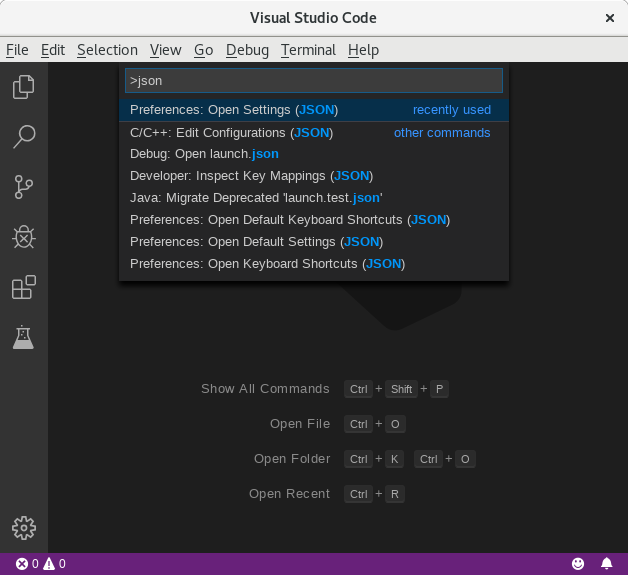
\includegraphics[width=.85\textwidth]{SelectJSON}
	\caption{Acceso a la configuración (archivo \texttt{settings.json}).}
	\label{preferences}
\end{figure}

Para simplificar la generación del software, vamos a colocar todos los archivos en el mismo paquete de Java.  Para esto, debemos modificar el archivo \verb|settings.json|.  Se puede acceder de varias formas, pero la más simple es siguiendo estos pasos:
\begin{enumerate}
	\item Abrir el \emph{Command Palette} con \verb|Ctl+Shift+P|,
	\item Buscar la opción \emph{Preferences: Open Settings (JSON)} y seleccionarla (Figura~\ref{preferences}),
	\item Agregar las siguientes líneas de código
	\begin{lstlisting}[style=consola]
	"antlr4.generation.mode": "external",
	"antlr4.generation.visitors": true
	\end{lstlisting}
\end{enumerate}
Hay que tener en cuenta que la coma es el separador en JSON y no debe faltar.  Además, las líneas de código deben estar antes de la llave de cierre como en el ejemplo del Código~\ref{settings}.

\lstinputlisting[float,style=consola,caption={Ejemplo de archivo \texttt{settings.json}.},label=settings]{settings.json}


\section{Primer Proyecto}
\label{primerproyecto}

Ya instalados y configurados los \emph{plug--ins} necesarios, podemos comenzar el primer proyecto.

\begin{figure}[t]
	\centering
	\begin{subfigure}[b]{.95\textwidth}
		\centering
		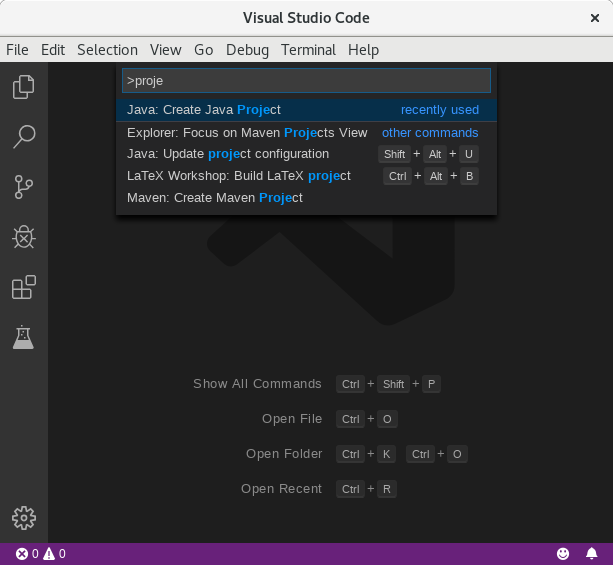
\includegraphics[width=.85\textwidth]{NuevoProyecto}
		\caption{Nuevo proyecto Java.}
		\label{maven_nuevo}
	\end{subfigure}
	\begin{subfigure}[b]{.95\textwidth}
		\centering
		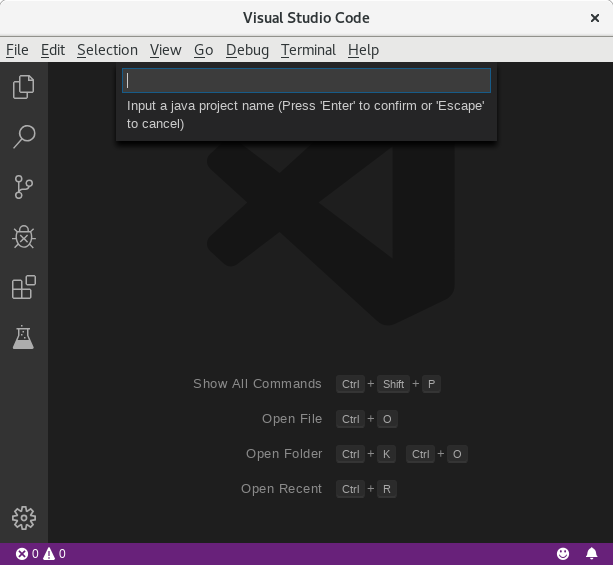
\includegraphics[width=.85\textwidth]{NombreProyecto}
		\caption{Nombre proyecto Java}
		\label{maven_nombre}
	\end{subfigure}
	\caption{Creación de un Proyecto Maven.}
	\label{maven}
\end{figure}

\begin{figure}[t]
	\centering
	\caption{Creación de un Proyecto Maven.}
	\label{maven_nombre}
\end{figure}

El primer paso es crear un proyecto Java.  Para esto, se puede acceder al \emph{Command Palette} con el atajo \verb|Ctl+Shift+P|, escribir la palabra \emph{project} y elegir la opción ``\emph{Java: Create Java Project}'' (Fig.~\ref{maven}). Luego, elegir la carpeta destino y darle nombre al proyecto (Fig.~\ref{maven}).



Los archivos de ANTLR llevan extensión \verb|*.g| o \verb|*.g4|, pero utilizaremos la segunda opción.




\end{document}
